\documentclass[journal]{IEEEtran}
\usepackage{graphicx}
\usepackage{amsmath}
\usepackage{amssymb}
\usepackage{hyperref}
\usepackage{float}
\usepackage{booktabs}
\usepackage{siunitx}
\usepackage{qrcode}

\title{Fresnel Double Mirror Experiment Report}
\author{{\large IBRAHIM H.I. ABUSHAWISH} \\ 
{\small Student ID: \hspace{1.5cm}. \\ 
Istanbul University, Dept. of Physics \\ 
Instructor: Res. Asst. Enes Talha KIRCA \\ 
Experiment Date: 25.04.2025, Submission Date: \\ 
Course \& Section Number: PHYS2405}
}
\markboth{Physics Laboratory Report, April 2025}{}

\begin{document}

\maketitle
\begin{abstract}
    This report presents the findings of the Fresnel Double Mirror experiment, conducted to measure the separation distance ($d$) between synchronized light sources using red ($\lambda = \SI{6040}{\angstrom}$) and green ($\lambda = \SI{5592}{\angstrom}$) light. The experiment utilizes the relationship between the fringe spacing ($\Delta x$), the distance to the screen ($L = \SI{56.1}{\centi\meter}$), and the wavelength ($\lambda$) of the light. The results were analyzed using Python, and the separation distances were calculated as \SI{0.0323}{\milli\meter} for red light and \SI{0.0314}{\milli\meter} for green light. The calculated values align with theoretical expectations, confirming the accuracy of the experimental measurements and analysis.
\end{abstract}

\section{Introduction}
The Fresnel Double Mirror experiment is a fundamental optical demonstration that illustrates the wave nature of light through interference phenomena. When coherent light encounters the double mirror system, it creates two virtual sources that produce an interference pattern, similar to Young's double-slit experiment.

\subsection{Theoretical Background}
The interference pattern produced by the Fresnel double mirror can be understood through the principle of wave superposition. When two coherent light waves from virtual sources $S_1$ and $S_2$ meet, they create alternating bright and dark fringes. The condition for constructive interference (bright fringes) occurs when the path difference is an integer multiple of the wavelength:
\begin{equation}
    \Delta r = m\lambda \quad (m = 0, \pm1, \pm2, ...)
\end{equation}

The relationship between the fringe spacing ($\Delta x$), wavelength ($\lambda$), distance to screen ($L$), and separation distance ($d$) is derived from geometric considerations:
\begin{equation}
    \Delta x = \lambda \frac{L}{d} \hspace{1cm} \cite{lab_manual}
\end{equation}

This can be rearranged to solve for the separation distance:
\begin{equation}
    d = \lambda \frac{L}{\Delta x}
\end{equation}


\section{Experimental Setup}
The experiment was conducted using the following parameters:
\begin{itemize}
    \item Wavelength of red light: \SI{6040}{\angstrom}
    \item Wavelength of green light: \SI{5592}{\angstrom}
    \item Distance to the screen ($L$): \SI{54.7}{\centi\meter} + \SI{1.4}{\centi\meter}
    \item Fringe spacing ($\Delta x$): Measured minimum and maximum values for both red and green light.
\end{itemize}

The experimental diagram is illustrated in Fig.~\ref{fig:setup_diagram}. The light source ($S$) emits coherent light, which passes through the Fresnel double mirror system, creating two virtual sources. The interference pattern is observed on the screen.

\begin{figure}[H]
    \centering
    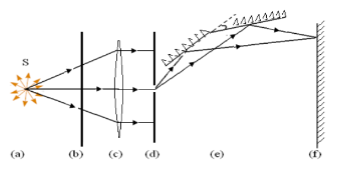
\includegraphics[width=0.8\linewidth]{../IMAGES/setup_diagram.png}
    \caption{Experimental setup diagram for the Fresnel Double Mirror experiment.}
    \label{fig:setup_diagram}
\end{figure}

The components of the setup are labeled as follows:
\begin{itemize}
    \item (a) Light source ($S$): Emits coherent light.
    \item (b) Color filter: Used to select specific wavelengths, such as green or red light.
    \item (c) Lens: Focuses the light onto the coherency slit.
    \item (d) Coherency slit: Ensures the light is coherent before reaching the Fresnel double mirror.
    \item (e) Fresnel double mirror: Splits the light into two virtual sources.
    \item (f) Screen: Where the interference fringes are recorded.
\end{itemize}

\begin{figure}[H]
    \centering
    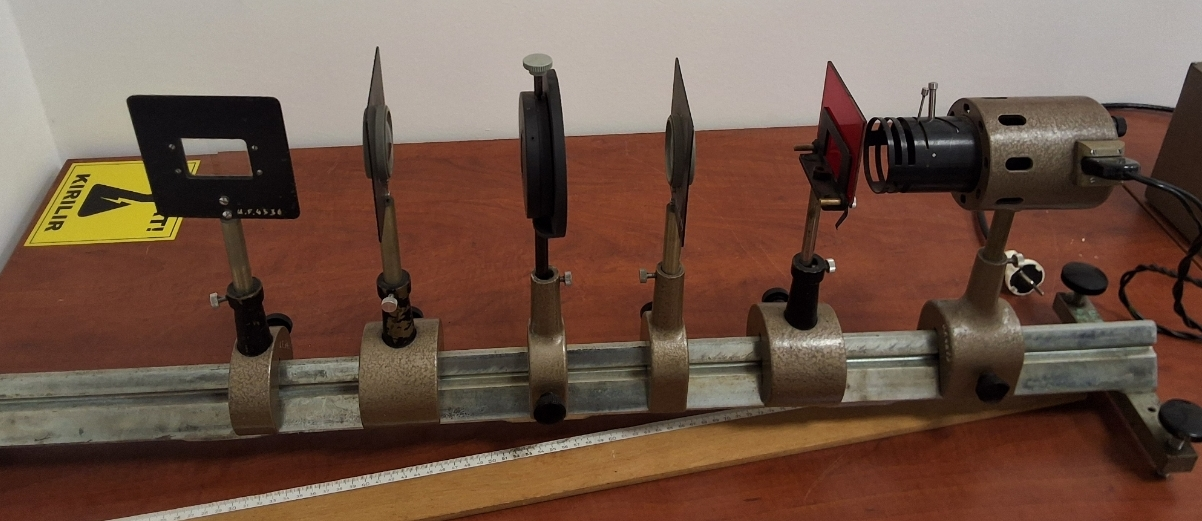
\includegraphics[width=0.8\linewidth]{../IMAGES/setup.jpg}
    \caption{Photograph of the experimental setup for the Fresnel Double Mirror experiment.}
    \label{fig:setup_photo}
\end{figure}

\section{Data and Calculations}
The average fringe spacing ($\Delta x_{\text{avg}}$) was calculated as the mean of the minimum and maximum fringe spacings. Using the formula for $d$, the separation distances were computed for both red and green light. The calculations were performed using Python, and the results are summarized below:
\begin{table}[H]
    \centering
    \caption{Calculated separation distances for red and green light.}
    \label{tab:separation_distances}
    \begin{tabular}{@{}ccc@{}}
        \toprule
        \textbf{Light Color} & \textbf{Wavelength (\si{\angstrom})} & \textbf{Separation Distance $d$ (\si{\milli\meter})} \\ \midrule
        Red                  & 6040                                & 0.0323                                             \\
        Green                & 5592                                & 0.0314                                             \\ \bottomrule
    \end{tabular}
\end{table}
\section{Results and Discussion}

The calculated separation distances for red and green light are \SI{0.0323}{\milli\meter} and \SI{0.0314}{\milli\meter}, respectively. The difference in $d$ values is attributed to the difference in wavelengths of the two light sources. The results are consistent with the theoretical relationship, demonstrating the validity of the experimental setup and calculations.

\subsection{Answers to Instructor's Questions}
\textbf{1. Why are the fringes not straight and not symmetric?} \\
The author of this report thinks that the fringes are not straight and symmetric due to imperfections in the alignment of the Fresnel double mirror system and the coherence of the light source. Additionally, slight variations in the mirror angle or surface quality can distort the interference pattern.

\textbf{2. Why did we use two different filters, and what happens if we use another filter?} \\
First of all, the imployment of any kind of filter was to produce a monochromatic light source to effectively study the impact of the wavelength as also the monochromatic light source is important for the absorvation of the interference with a sharper effect. Two different filters (red and green) was used to observe the effect of wavelength on the fringe spacing and separation distance. If another filter is used, the wavelength of the light will change, leading to a corresponding change in the fringe spacing and calculated separation distance, as per the relationship $\Delta x = \lambda \frac{L}{d}$.
\textbf{3. What happens if the angle between the mirrors is increased?} \\

In Fresnel's double mirror experiment, increasing the angle between the mirrors causes several effects:
\begin{itemize}
    \item \textbf{Increase in virtual source separation ($d$):} As the mirror angle ($\alpha$) increases, the separation $d$ between the virtual images grows approximately linearly for small angles.
    
    \item \textbf{Decrease in fringe spacing ($\Delta x$):} The fringe spacing, given by
    \[
    \Delta x = \lambda \frac{L}{d},
    \]
    decreases as $d$ increases, resulting in narrower fringes.
    
    \item \textbf{Reduction in spatial coherence:} A larger $d$ reduces spatial coherence. When the path difference exceeds the coherence length, fringe visibility diminishes significantly \cite{mustansiriyah_wavefront}.
    
    \item \textbf{Disappearance of the interference pattern:} At sufficiently large angles:
    \begin{itemize}
        \item The fringe spacing becomes too fine to resolve.
        \item The overlap region between the beams shrinks.
        \item Coherence is lost, and interference vanishes entirely \cite{mustansiriyah_wavefront}.
    \end{itemize}
\end{itemize}

Thus, stable interference requires both adequate spatial coherence and sufficient beam overlap.

\section{Conclusion}
The Fresnel Double Mirror experiment successfully demonstrated the relationship between fringe spacing, wavelength, and separation distance. The calculated values for $d$ align with theoretical expectations, confirming the accuracy of the experimental measurements and analysis.

\section{Experiment Photos}
The following images were taken during the experiment to document the setup and the observed interference pattern for red filtered light configurations.
The first image shows the initial alignment of the Fresnel double mirror system, while the second image captures the interference fringes observed on the screen.:

\begin{figure}[H]
    \centering
    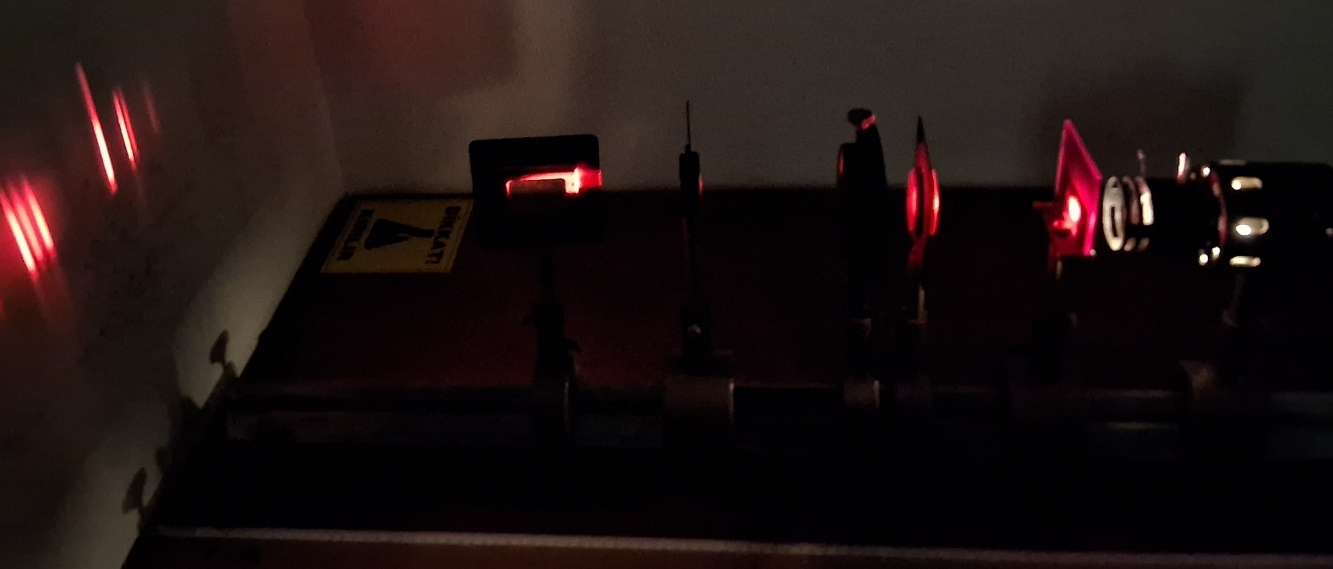
\includegraphics[width=0.8\linewidth]{../IMAGES/setup_opened.jpg}
    \caption{Initial alignment of the Fresnel double mirror system.}
    \label{fig:photo1}
\end{figure}

\begin{figure}[H]
    \centering
    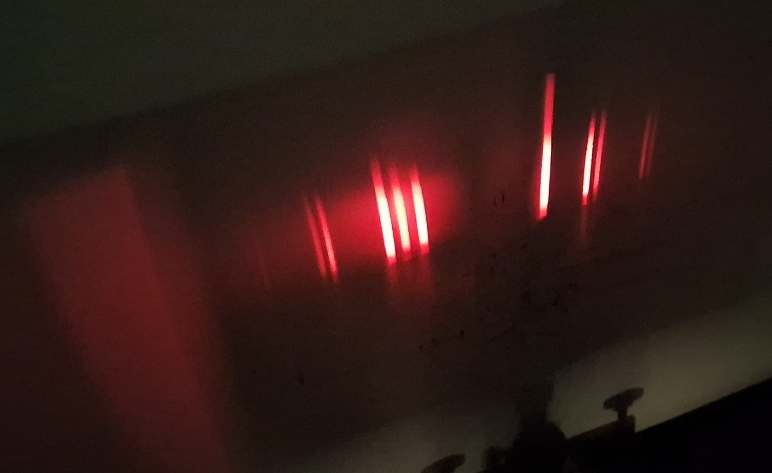
\includegraphics[width=0.8\linewidth]{../IMAGES/pattern.jpg}
    \caption{Observation of interference fringes on the screen.}
    \label{fig:photo2}
\end{figure}

\section{Additional Resources}
For detailed information, including the Lab Manual, source code, and related experiments, visit the GitHub repository provided below or scan the QR code in Fig.~\ref{fig:qr_code} \cite{github}.

\begin{figure}[H]
    \centering
    \begin{minipage}{0.15\textwidth}
        \centering
        \qrcode[height=2cm]{https://github.com/ibeuler/LAB-Reports}
    \end{minipage}%
    \begin{minipage}{0.2\textwidth}
        \raggedright
        \caption{Access the GitHub repository for the lab manual, source code, and related experiments: \href{https://github.com/ibeuler/LAB-Reports}{\url{https://github.com/ibeuler/LAB-Reports}}.}
        
        \label{fig:qr_code}
    \end{minipage}
\end{figure}

\bibliographystyle{plain}
\bibliography{references}

\end{document}